\documentclass[aspectratio=169,10pt,t]{beamer}
% \usetheme[
% %%% options passed to the outer theme
% %    progressstyle=fixedCircCnt,   %either fixedCircCnt, movCircCnt, or corner
% %    rotationcw,          % change the rotation direction from counter-clockwise to clockwise
% %    shownavsym          % show the navigation symbols
%   ]{SDUsimple}
\usepackage{SDUtheme/beamerthemeSDUsimple}
% If you want to change the colors of the various elements in the theme, edit and uncomment the following lines
% Change the bar and sidebar colors:
%\setbeamercolor{SDUsimple}{fg=red!20,bg=red}
%\setbeamercolor{sidebar}{bg=red!20}
% Change the color of the structural elements:
%\setbeamercolor{structure}{fg=red}
% Change the frame title text color:
%\setbeamercolor{frametitle}{fg=blue}
% Change the normal text color background:
%\setbeamercolor{normal text}{fg=black,bg=gray!10}
% ... and you can of course change a lot more - see the beamer user manual.
\usepackage{color}
\usepackage{float}
\usepackage{dsfont}                         % Enables double stroke fonts
\usepackage{bm}
\usepackage[utf8]{inputenc}
\usepackage[english]{babel}
\usepackage[T1]{fontenc}
\usepackage{listings}
\usepackage{amsmath}
\usepackage{import}
% Or whatever. Note that the encoding and the font should match. If T1
% does not look nice, try deleting the line with the fontenc.
\usepackage{helvet}
\usefonttheme{professionalfonts}

\newtheorem{algorithm}{Algorithm}
%\newtheorem{problem}{Problem}
\newtheorem{proposition}{Proposition}
% colored hyperlinks
\newcommand{\chref}[2]{%
    \href{#1}{{\usebeamercolor[bg]{SDUsimple}#2}}%
}

\title{Multivariate data and multivariate normal distribution}
\subtitle{Multivariate Statistic}
%\date{\today}
\date{ }

\author{
    Made by: \\
    \textbf{Lasse Gøransson, Marc Evald, Anne-Charlotte Poulsen \& Aske Møller}
}

% - Give the names in the same order as they appear in the paper.
% - Use the \inst{?} command only if the authors have different
%   affiliation. See the beamer manual for an example

\institute[
%  {\includegraphics[scale=0.2]{SDU_segl}}\\ %insert a company, department or university logo
SDU Robotics\\
The Maersk Mc-Kinney Moller Institute\\
University of Southern Denmark
] % optional - is placed in the bottom of the sidebar on every slide
{% is placed on the bottom of the title page
    SDU Robotics\\
    The Maersk Mc-Kinney Moller Institute\\
    University of Southern Denmark

    %there must be an empty line above this line - otherwise some unwanted space is added between the university and the country (I do not know why;( )
}

% specify a logo on the titlepage (you can specify additional logos an include them in
% institute command below
\pgfdeclareimage[height=0.5cm]{titlepagelogo}{SDUgraphics/SDU_logo_new} % placed on the title page
%\pgfdeclareimage[height=1.5cm]{titlepagelogo2}{SDUgraphics/SDU_logo_new} % placed on the title page
\titlegraphic{% is placed on the bottom of the title page
    \pgfuseimage{titlepagelogo}
    %  \hspace{1cm}\pgfuseimage{titlepagelogo2}
}

\begin{document}
% the titlepage
{\SDUwavesbg%
    \begin{frame}[plain,noframenumbering] % the plain option removes the header from the title page
        \titlepage
\end{frame}}
%%%%%%%%%%%%%%%%

% TOC
%%%%%%%%%%%%%%%

\begin{frame}[t]
    \frametitle{Agenda}
    
    \begin{itemize}
        \item Univariate $\rightarrow$ Multivariate
        \item Multivariate theory 
        \item Multivariate sampling
        \item MVN
        \item Model Check
    \end{itemize}
\end{frame}


\begin{frame}[t]
    \frametitle{Univariate Statistics}
    Univariate\\

    \begin{itemize}
        \item Stochastic Variable
        \item Mean
        \item Variance
    \end{itemize}

\end{frame}

\begin{frame}[t]
    \frametitle{Multivariate}
    \framesubtitle{Theory}
    \begin{itemize}
        \item<only@1> Stochastic Variable
            \[
                \underset{p\times 1}{X}
            \] 
        \item Mean
            \[
                E \left[ X \right] =
                \underset{p\times 1}{\mu} =
                \begin{bmatrix}
                    E \left[ X_1  \right] \\
                    \vdots\\
                    E \left[ X_p  \right] 
                \end{bmatrix}
            \] 
        \item Variance
            \[
                V \left[ X  \right]  =
                \underset{p\times p}{\Sigma}
                =
                \begin{bmatrix}
                    \sigma_1^{2} & \sigma_{12} & \cdots & \sigma_{1p}\\
                                 & \sigma_2^{2} & &\\
                                 & & \ddots &\\
                                 &&& \sigma_{p}^{2}
                \end{bmatrix}
            \] 
					\item<2> Correlation
						\[
						\rho = \begin{bmatrix}
							1 & \rho_{12} & \cdots & \rho_{1p}\\
								& \ddots& & \rho_{2p}\\
								&&&\\
								& & &1
						\end{bmatrix}
						\] 
    \end{itemize}
\end{frame}


\begin{frame}[t]
    \frametitle{Sampling}
    \begin{itemize}
        \item Data
            \[
                x = 
                \begin{bmatrix}
                    \begin{bmatrix}
                        x_{11} & \cdots & x_{1p}
                    \end{bmatrix}\\
                    \vdots\\
                    \begin{bmatrix}
                        x_{n1} & \cdots & x_{np}
                    \end{bmatrix}\\
                \end{bmatrix}
            \] 
        \item Estimated Mean
            \[
                \hat{\mu} = \bar{x} = 
                \begin{bmatrix}
                    \frac{1}{n} \sum^{n}_{j=1} x_{j1}\\
                    \vdots\\
                    \frac{1}{n} \sum^{n}_{j=1} x_{jp}
                \end{bmatrix}
            \] 
        \item Estimated Variance
            \[
                \hat{\Sigma} = S = 
                \frac{1}{n-1} \sum^{n}_{j=1} 
                \left( x_j - \bar{x}  \right) 
                \left( x_j - \bar{x}  \right) ^{T}
            \] 
				\item Estimated Correlation
					\[
					\hat{\rho} = R
					\rightarrow
					r_{ij} = \frac{s_{ij}}{\sqrt{s_{ii} s_{jj}}} 
					\] 
    \end{itemize}
\end{frame}


\begin{frame}[t]
    \frametitle{MVN}

    Multivariate Normal Distribution
    \[
        \underset{p\times1}{X} \sim N_p(\mu, \Sigma)
    \] 
    \begin{figure}[H]
        \centering
				\import{images/}{mvn-3d.pdf_tex}
    \end{figure}

\end{frame}

\begin{frame}[t]
	\frametitle{MVN}
	\framesubtitle{Contours}
	\begin{figure}[h]
		\centering
		\import{images/}{mvn.pdf_tex}
	\end{figure}
	\pause
    \begin{itemize}
        \item Mahalanobis Distance $(x - \mu)^T \Sigma^{-1} (x - \mu)\sim \chi^2_p$
    \end{itemize}
\end{frame}

\begin{frame}[t]
    \frametitle{Model Check}

    \begin{columns}
        \begin{column}{0.5\textwidth}
            \begin{figure}[H]
                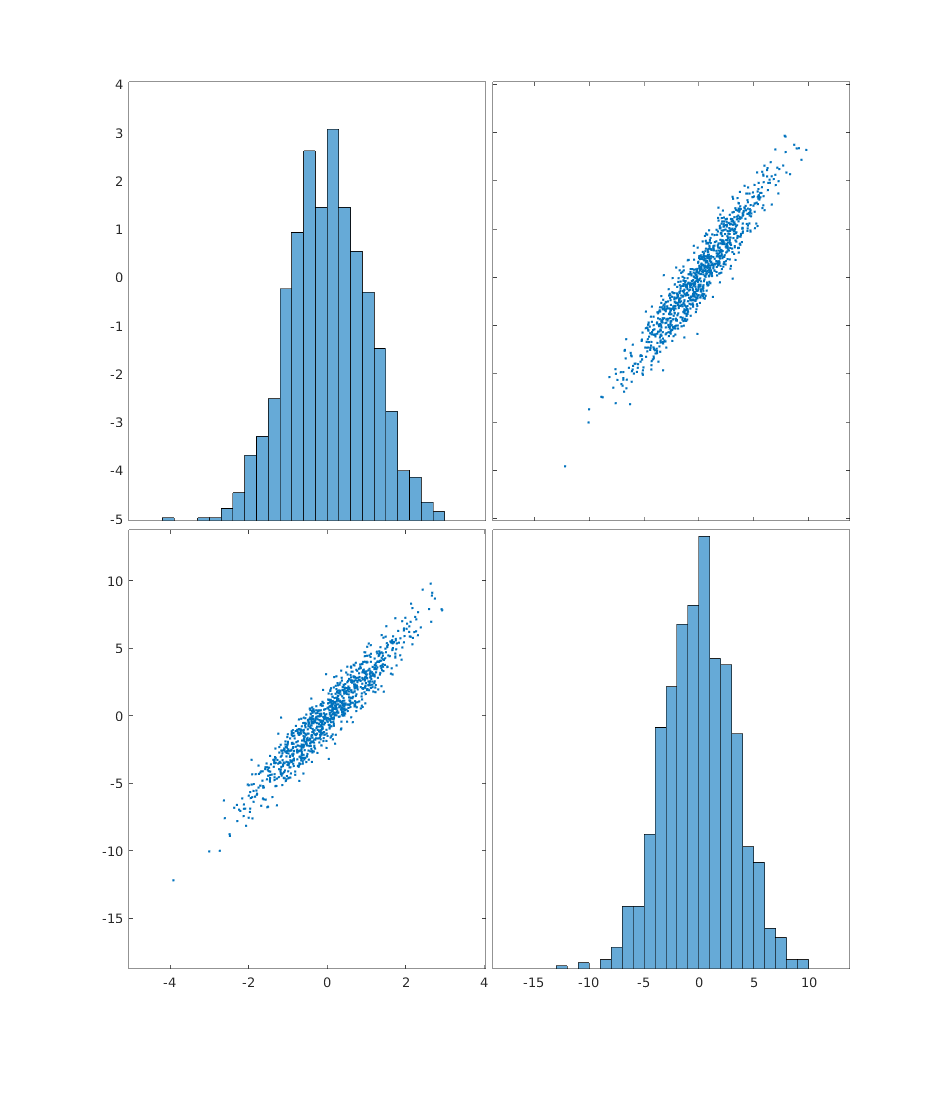
\includegraphics[scale=0.2]{images/scatterplotCorr.png}
            \end{figure} 
        \end{column}
        \begin{column}{0.5\textwidth}
            \begin{figure}[H]
                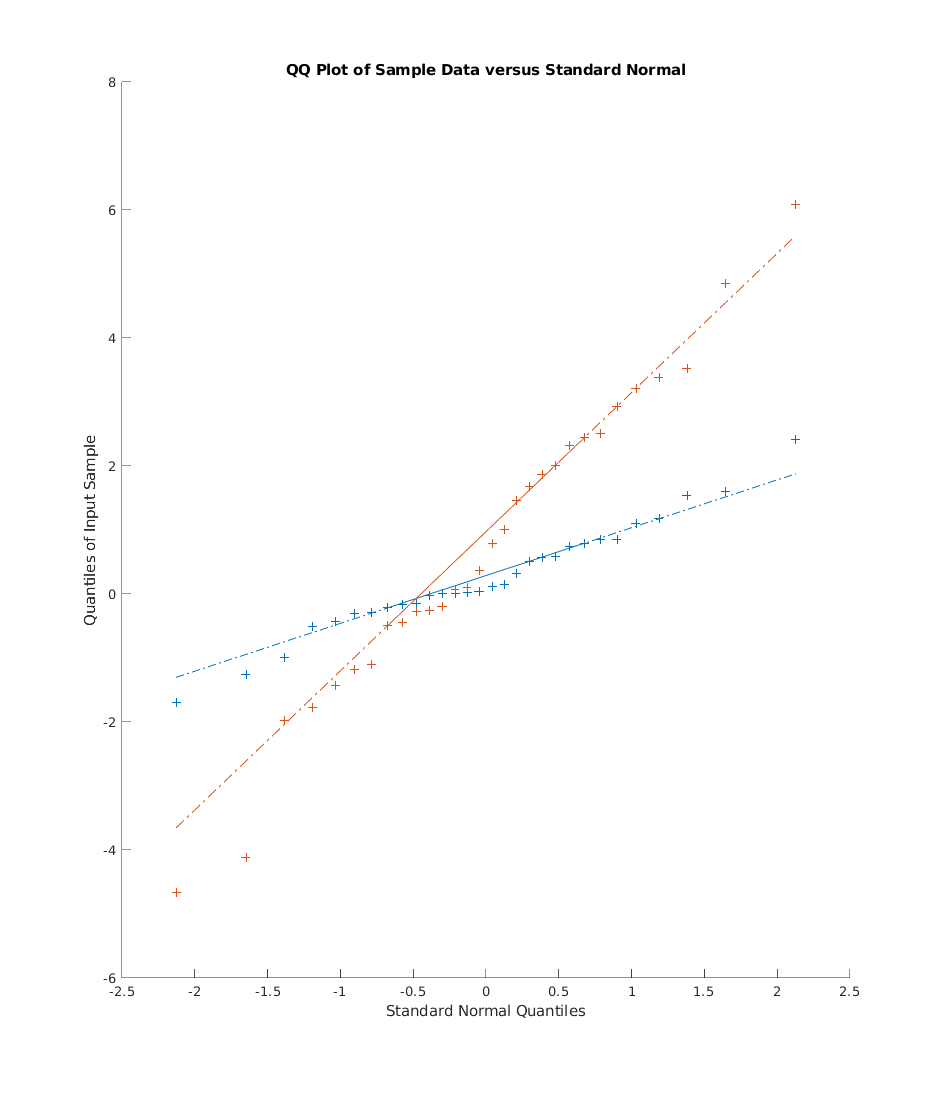
\includegraphics[scale=0.2]{images/qq.png}
            \end{figure}    
        \end{column}
    \end{columns}

\end{frame}


\end{document}
